\documentclass[t]{beamer}

% Load general definitions
% Preamble file - general definitions, package loading, etc.

%=================================
% Load packages
\usepackage{amssymb,amsmath}
\usepackage{graphicx}
\usepackage{url}
\usepackage{tikz}
\usetikzlibrary{mindmap,trees,arrows}
\usepackage{fancyvrb}
\usepackage[english]{babel}
\usepackage[latin1]{inputenc}
\usepackage{subfigure}
\usepackage{times}
\usepackage[T1]{fontenc}
\usepackage{cancel}
\usepackage{color}
\usepackage{listings}

%=================================
% Set mode
\mode<presentation>
{
	\usetheme{Madrid}
	\usecolortheme{whale}
	\useoutertheme{infolines}
	\setbeamercovered{invisible}
}

% Get rid of nav bar
\beamertemplatenavigationsymbolsempty

% Insert frame number at bottom of the page.
\usefoottemplate{\hfil\tiny{\color{black!90}\insertframenumber}} 

%=================================
% Define new commands

\newcommand\Real{{\mathbb{R}}}
%\newcommand{\vi}{\vspace{0.6\baselineskip}}
%\newcommand{\goodgap}{\hspace{\subfigtopskip}\hspace{\subfigbottomskip}}


% Equation environments
\newcommand{\beq}{\begin{equation}}
\newcommand{\eq}{\end{equation}}
\newcommand{\beqs}{\begin{equation*}}
\newcommand{\eqs}{\end{equation*}}
\newcommand{\beqn}{\begin{eqnarray}}
\newcommand{\eqn}{\end{eqnarray}}

% Bold variables
\newcommand{\mbf}[1]{\ensuremath{\mathbf{#1}}}

% Itemization
\newcommand{\bitem}{\begin{itemize}}
\newcommand{\eitem}{\end{itemize}}
\newcommand{\spitem}{\vskip 1em\item}
\newcommand{\bitems}{\begin{itemize}\item}
\newcommand{\benums}{\begin{enumerate}\item}
\newcommand{\eenum}{\end{enumerate}}

% color blocks
\newenvironment{colorblock}[2]{%
\setbeamercolor{block title}{#2}
\begin{block}{#1}}{\end{block}}

% Vertical spacing
\newcommand{\vone}{\vskip 1em}
\newcommand{\vhalf}{\vskip .5em}

% Frame environments
\newenvironment{ftst}[3][t]{%
\begin{frame}{environment=ftst,#1}
\frametitle{#2}
\framesubtitle{#3}}{\end{frame}}

\newenvironment{ftstf}[2]{
\begin{frame}[fragile,environment=ftstf]
\frametitle{#1}
\framesubtitle{#2}}{\end{frame}}

% colors
\definecolor{MyGray}{rgb}{0.5,0.5,0.5}
\definecolor{MyDBGray}{rgb}{0.1,0.1,0.4}
\definecolor{darkgreen}{rgb}{0,0.4,0}
\definecolor{black}{rgb}{0,0,0}
\def\defn#1{{\color{red} #1}}

% Footnote
\renewcommand{\thefootnote}{\alph{footnote}}

% Relaxed footnotes
\newcommand{\lfr}[1]{\let\thefootnote\relax\footnote{\tiny #1}}

% Verbatim environment - using FANCYVRB package
\DefineVerbatimEnvironment%
{rcode}{Verbatim}
{fontsize=\scriptsize}

% Verbatim environment - using LISTINGS package
%\lstnewenvironment{rcode} {\lstset{	language = R,
%									basicstyle = \scriptsize\ttfamily,
%									showspaces = false,
%									showstringspaces = false,
%									showtabs = false,
%									keywordstyle = \color{black}\bfseries,
%									commentstyle = \color{darkgreen},
%									numbers = none,
%									otherkeywords={	<-,
%													ggplot,
%													geom_boxplot,
%													facet_grid,
%													shapiro.test,
%													fligner.test,
%													glht,
%													with},
%									deletekeywords={data,
%													model,
%													residuals,
%													c,
%													axis,
%													default,
%													labels,
%													qq.text}}}%
%{}


% Specific definitions
\title[]{Design and Analysis of Experiments}
\subtitle[]{12 - Factorial Designs}
\author[]{Felipe Campelo\\{\footnotesize http://www.cpdee.ufmg.br/\textasciitilde fcampelo}}
\institute{Graduate Program in Electrical Engineering}
\date{\scriptsize Belo Horizonte\\May 2015}

\begin{document}

% cover page
\setbeamertemplate{footline}{}
\begin{frame}
\begin{flushright}

\includegraphics[width=.25\textwidth]{../figs/principal_completa3_ufmg}
\end{flushright}
  \titlepage
  \begin{tikzpicture}[remember picture,overlay]
  \node[anchor=south east,xshift=-5pt,yshift=122pt] at (current page.south east) {\tiny Version 2.11};
  \node[anchor=south west,yshift=0pt] at (current page.south west) {
\includegraphics[width=.15\textwidth]{../figs/by-nc-sa.png}};
  \end{tikzpicture}  
\end{frame}

%=====

% quotation page
  \begin{frame}[b]
		\frametitle{}
\begin{columns}[T]
\column{0.77\textwidth}
\flushright{\small ``\textit{We did not evolve to understand or\\
comprehend reality. We evolved to survive it.\\
For understanding we need science.}''
\vskip 4.5em
Mark A. Crislip\\
1952-\\
American infectologist\\}
\column{0.23\textwidth}
\begin{tikzpicture}[remember picture,overlay]
\node[anchor=south east,yshift=23pt,xshift=0pt] at (current page.south east)
{
\includegraphics[width=\textwidth]{../figs/markcrislip.jpg}};
\end{tikzpicture}
\end{columns}
\vhalf
\lfr{Image: \url{http://boards.medscape.com/.29f3af03/}}
\end{frame}

%=====
% Main slides

\begin{ftst}
{Factorial Designs}
{Basic definitions}
Many experiments involve more than a single \textit{factor} of interest - that is, multiple independent variables that can influence a response variable.
\vone
In general, an effective way to explore the main effects and interactions of multiple factors is the use of a \textit{factorial design} in which all level combinations are evaluated at each experimental replicate;
\vone
In this context, the \textbf{main effect} of a factor quantifies the mean change in the response variable due to changing between the levels of that factor;
\vone
An \textbf{interaction effect} represents the mean change in the response variable due to the simultaneous change of levels of two or more factors.
\end{ftst}

%=====

\begin{ftst}
{Factorial Designs}
{Example: Electrical current in motors}
\begin{columns}
\column[T]{0.2\textwidth}
\vspace{-1.5em}\ \ \ 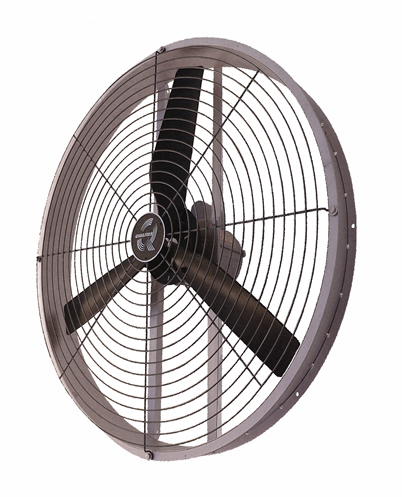
\includegraphics[width=.8\textwidth]{../figs/ventilador.png}
\column[T]{0.8\textwidth} Two engineers wish to investigate factors that may affect the electrical current demanded by the single-phase motors used for ventilation in an industrial chicken coop.
\end{columns}
\vhalf
Previous observations suggest that the current varies considerably from motor to motor, and process knowledge suggests two likely candidates for explaining this variability: the \textit{Manufacturer} (A, B or C) and the \textit{State} (original or rewinded) of each motor.
\vone
To investigate this question, the engineers decide to sample 40 motors from each manufacturer, with 20 in the original state and 20 being rewinded motors.
\lfr{Adapted from M.H.Costa and T.L. Vieira's course project for the Design and Analysis of Experiments Course, PPGEE-UFMG, November 2013. The data used in this example is not necessarily the original one.}
\lfr{Image: \url{http://refrigelms.com.br/ventilador-para-aviario-qla85-grade-p-1734.html}}
\end{ftst}

%=====

\begin{ftstf}
{Exploratory data analysis}
{Example: Electrical current in motors}
\begin{rcode}
> data <- read.table("../data files/motors.txt", header = TRUE)
> library(ggplot2)
> p <- ggplot(data, aes(x = Manufacturer, y = Current.Amperes, fill = Manufacturer))
> p + geom_boxplot() + facet_grid(.~State) + ...
\end{rcode}

\begin{tikzpicture}[remember picture,overlay]
\node[anchor=south,yshift=0pt,xshift=0pt] at (current page.south)
{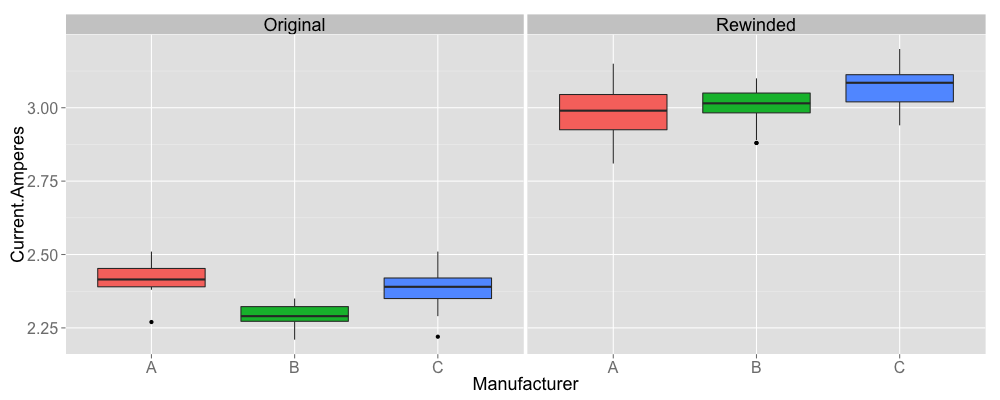
\includegraphics[width=\textwidth]{../figs/motors_box1.png}};
\end{tikzpicture}
\end{ftstf}

%=====

\begin{ftst}
{Factorial Designs}
{Example: Electrical current in motors}
The exploratory plot suggests a relatively large effect for the \textit{State} factor, but is inconclusive with regards to the \textit{Manufacturer} effect. Any interaction effect is also likely to by small.
\vhalf
Lets assume for this example that the engineers want $\alpha = 0.05$, $\beta = 0.2$ and $\delta^* = 0.1 A$.
\begin{tikzpicture}[remember picture,overlay]
\node[anchor=south,yshift=0pt,xshift=0pt] at (current page.south)
{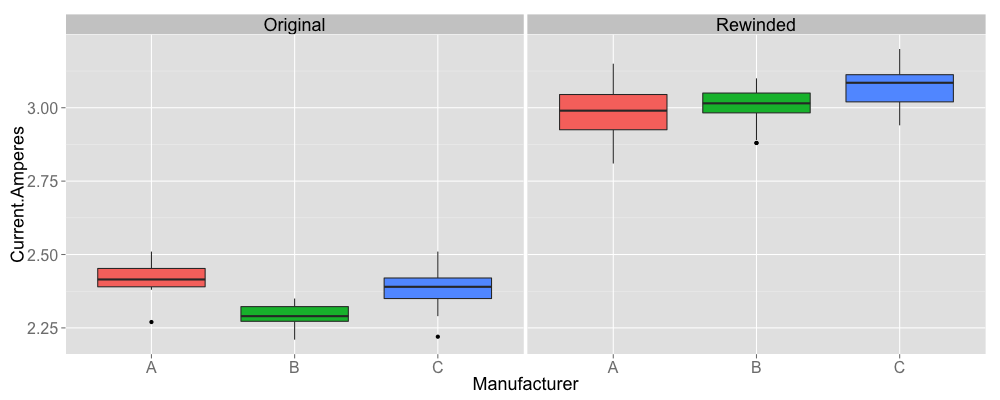
\includegraphics[width=\textwidth]{../figs/motors_box1.png}};
\end{tikzpicture}
\end{ftst}

%=====

\begin{ftst}
{Factorial Designs}
{Statistical model for two factors}
In the general case for a completely randomized factorial design we have:

\bitems \textit{a} levels for factor \textbf{A};
\item \textit{b} levels for the factor \textbf{B};
\item \textit{n} replicates within each combination of levels;
\item Completely randomized collection of observations;
\eitem

The effects model for a set of observations collected following this design can be expressed as:

\beqs y_{ijk} = \mu+\tau_i+\beta_j+(\tau\beta)_{ij}+\epsilon_{ijk}\begin{cases}
i=1,\ldots,a\\
j=1,\ldots,b\\
k=1,\ldots,n
\end{cases}\eqs
\end{ftst}

%=====

\begin{ftst}
{Factorial Designs}
{Statistical model for two factors}
\beqs y_{ijk} = \mu+\tau_i+\beta_j+(\tau\beta)_{ij}+\epsilon_{ijk}\begin{cases}
i=1,\ldots,a\\
j=1,\ldots,b\\
k=1,\ldots,n
\end{cases}\eqs
\vone
As before, effects are treated as deviations from the grand mean.\\By construction:
\vhalf
\beqs \sum\limits_{i=1}^{a}\tau_i=0\ \ \ \ \ \ \ \ \ \ \ \ \ \ \ \ \ \ \sum\limits_{j=1}^{b}\beta_j=0\eqs
\vhalf
\beqs \sum\limits_{i=1}^{a}(\tau\beta)_{ij} = \sum\limits_{j=1}^{b}(\tau\beta)_{ij} = 0\eqs
\end{ftst}

%=====

\begin{ftst}
{Factorial Designs}
{Statistical model for two factors}
The factorial design emerges whenever we wish to model both the main and the interaction effects of multiple factors. This means that, for the two-factor case, the hypotheses that can be tested are:

\begin{align*}
\mbox{Factor $A$, main effect:}&\begin{cases}
H_0: \tau_i = 0,\ \forall i\\
H_1: \exists\tau_i \neq 0\\
\end{cases}\\
& \\
\mbox{Factor $B$, main effect:}&\begin{cases}
H_0: \beta_j = 0,\ \forall j\\
H_1: \exists\beta_j \neq 0\\
\end{cases}\\
& \\
\mbox{Interaction effect, $AB$:}&\begin{cases}
H_0: (\tau\beta)_{ij} = 0,\ \forall i,j\\
H_1: \exists(\tau\beta)_{ij} \neq 0\\
\end{cases}
\end{align*}
\end{ftst}

%=====

\begin{ftst}
{Factorial Designs}
{Statistical model for two factors}
The test statistics for these hypotheses will, as usual, be derived from the partition of the total variability into specific components:
\begin{align*}
SST &= \sum\limits_{i=1}^{a}\sum\limits_{j=1}^{b}\sum\limits_{k=1}^{n}\left(y_{ijk} - \bar{y}_{\cdot\cdot\cdot}\right)^2\\
&= \underbrace{bn\sum\limits_{i=1}^{a}\left(\bar{y}_{i\cdot\cdot} - \bar{y}_{\cdot\cdot\cdot}\right)^2}_{SS_A} + \underbrace{an\sum\limits_{j=1}^{b}\left(\bar{y}_{\cdot j\cdot} - \bar{y}_{\cdot\cdot\cdot}\right)^2}_{SS_B}\\
&+\underbrace{n\sum\limits_{i=1}^{a}\sum\limits_{j=1}^{b}\left(\bar{y}_{ij\cdot} -\bar{y}_{i\cdot\cdot}-\bar{y}_{\cdot j\cdot}+ \bar{y}_{\cdot\cdot\cdot}\right)^2}_{SS_{AB}} + \underbrace{\sum\limits_{i=1}^{a}\sum\limits_{j=1}^{b}\sum\limits_{k=1}^{n}\left(y_{ijk} - \bar{y}_{ij\cdot}\right)^2}_{SS_E}
\end{align*}
\lfr{To distinguish $SS_{AB}$ from $SS_{E}$ we need $n\geq 2$.}
\end{ftst}

%=====

\begin{ftst}
{Factorial Designs}
{Statistical model for two factors}
The mean squares are also calculated as usual:
\begin{align*}
MS_A		&= \frac{SS_A}{a-1} 				& E\left[MS_A\right] 	& = \sigma^2 + \frac{bn\sum\limits_{i=1}^{a}\tau_i^2}{a-1}\\
MS_B		&= \frac{SS_B}{b-1} 				& E\left[MS_B\right] 	& = \sigma^2 + \frac{an\sum\limits_{j=1}^{b}\beta_j^2}{b-1}\\
MS_{AB} 	&= \frac{SS_{AB}}{(a-1)(b-1)}	&E\left[MS_{AB}\right] & =\sigma^2 + \frac{n\sum\limits_{i=1}^{a}\sum\limits_{j=1}^{b}(\tau\beta)_{ij}^2}{(a-1)(b-1)}\\
\ \\
MS_E 		&= \frac{SS_E}{ab(n-1)}			&E\left[MS_E\right] 	&= \sigma^2\\
\end{align*}
\end{ftst}

%=====

\begin{ftst}
{Factorial Designs}
{Statistical model for two factors}
If the usual assumptions ($\epsilon_{ijk}$ i.i.d. $\mathcal{N}(0, \sigma^2)$) hold, the fractions:

\begin{align*}
F_0^{(A)} &= \frac{MS_A}{MS_E}\\
\ \\
F_0^{(B)} &= \frac{MS_B}{MS_E}\\
\ \\
F_0^{(AB)} &= \frac{MS_{AB}}{MS_E}
\end{align*}
\vhalf

are distributed under their respective null hypotheses as $F$ variables (each with their respective degrees of freedom), and the hypotheses can be tested in the usual manner (i.e., comparing the obtained value of $F_0$ against the critical value of $F_{\alpha;df_1;df_2}$).
\end{ftst}

%=====

\begin{ftstf}
{Example: Electrical current in motors}
{Statistical model for two factors}
\begin{rcode}
> model <- aov(Current.Amperes~State*Manufacturer,
+              data = data)
> summary(model)
                    Df Sum Sq Mean Sq F value   Pr(>F)    
State                1 12.956  12.956 2798.41  < 2e-16 ***
Manufacturer         2  0.118   0.059   12.71 1.04e-05 ***
State:Manufacturer   2  0.114   0.057   12.27 1.49e-05 ***
Residuals          114  0.528   0.005                     
---

> summary.lm(model)$r.squared
[1] 0.9615174
\end{rcode}
\end{ftstf}

%=====

\begin{ftstf}
{Example: Electrical current in motors}
{Statistical model for two factors}
As usual, the assumptions can be verified by means of residual analysis, like in the one-way ANOVA (except for a little adjustment needed for the Fligner-Killeen test)
\vhalf
\begin{rcode}
> shapiro.test(model$residuals)
W = 0.9857, p-value = 0.2392

> fligner.test(Current.Amperes ~ interaction(State, Manufacturer), 
+              data = data)
med chi-squared = 10.1721, df = 5, p-value = 0.0705
\end{rcode}
\begin{tikzpicture}[remember picture,overlay]
\node[anchor=south east,yshift=0pt,xshift=0pt] at (current page.south east)
{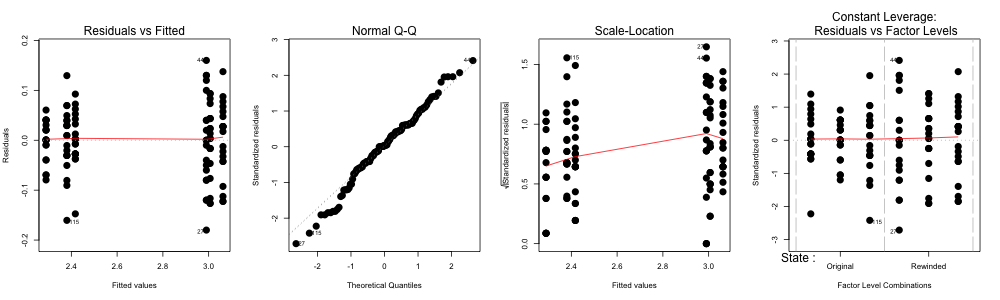
\includegraphics[width=\textwidth]{../figs/motors_res.png}};
\end{tikzpicture}
\end{ftstf}

%=====

\begin{ftst}
{Factorial designs}
{Multiple Comparisons}
If the ANOVA indicates the existence of significant effects, we can perform pairwise comparisons between levels to investigate specific differences;
\vhalf
When the interaction effect is not significant, the comparisons between factor levels can be done in a straightforward manner, using the estimated level means. For instance, the test statistic for comparing the means of levels 2 and 3 of factor A could be calculated as:
\beqs
t_0 = \frac{\bar{y}_{2\cdot\cdot} - \bar{y}_{3\cdot\cdot}}{\sqrt{2\frac{MS_E}{n'}}}
\eqs
\vhalf
\noindent where $n'$ is the number of specific replicates for the comparison under consideration.
\end{ftst}

%=====

\begin{ftstf}
{Factorial designs}
{Multiple Comparisons}
More generally,
\beqs
t_0 = \frac{\Delta\bar{y}}{\sqrt{2\frac{MS_E}{n'}}}
\eqs
\vhalf
For comparisons of factor levels (main effects), the value of $n'$ is the total number of observations under that level;
\vhalf
For comparisons of level combinations (interaction effects), it is the number of observations within each combination group;
\vhalf
\begin{rcode}
> replications(Current ~ State*Manufacturer,
+              data = data)
             State       Manufacturer State:Manufacturer 
                60                 40                 20 
\end{rcode}
\vhalf
Also, the $\alpha$ value for the comparisons has to be adjusted to prevent inflation of the type-I error rate.
\end{ftstf}

%=====

\begin{ftstf}
{Factorial designs}
{Multiple Comparisons}
The usual routines for performing multiple comparisons in \textit{R} are applicable. For instance, performing \textit{all vs all} comparisons using Tukey's method yields, for the \textit{Manufacturer} factor:
\vhalf
\begin{rcode}
> mcp.manuf <- glht(model, linfct = mcp(Manufacturer = "Tukey"))
Warning message:
In mcp2matrix(model, linfct = linfct) :
  covariate interactions found 
  -- default contrast might be inappropriate

> plot(confint(mcp.manuf),
+      cex.axis   = 1.2,
+      cex        = 2)
\end{rcode}
\begin{tikzpicture}[remember picture,overlay]
\node[anchor=south east,yshift=0pt,xshift=0pt] at (current page.south east)
{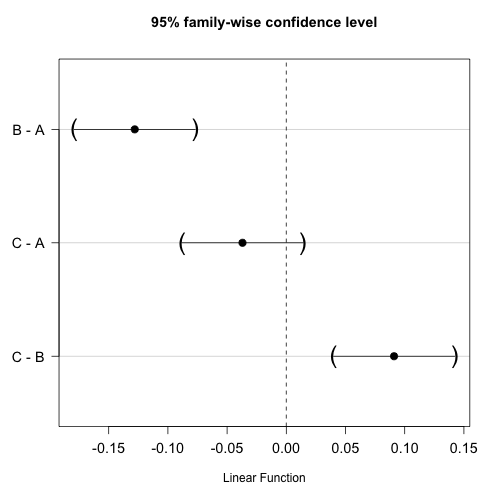
\includegraphics[width=.4\textwidth]{../figs/motors_mcpManuf.png}};
\end{tikzpicture}
\end{ftstf}

%=====

\begin{ftstf}
{Factorial designs}
{Multiple Comparisons}
The comparison of means for the interaction groups requires a little more work, but nothing too complex. Here, we assume that we want to compare all groups versus the one with the smallest sample average.
\vhalf
\begin{rcode}
> # Create meta-factor for interaction groups
> interfac <- with(data, 
+                  interaction(State, Manufacturer))
> 
> # Use group with the smallest sample mean as the reference
> with(data, which.min(tapply(Current.Amperes, interfac, mean)))
Original.B 
         3 
> interfac <- relevel(interfac, ref = "Original.B")
> 
> # ReFit model
> model2 <- aov(Current.Amperes ~ interfac,
+               data = data)
> 
> # Multiple comparisons
> mcp.inter <- glht(model2,
+                 linfct = mcp(interfac = "Dunnett"))
\end{rcode}
\end{ftstf}

%=====

\begin{ftstf}
{Factorial designs}
{Multiple Comparisons}
\begin{rcode}
> par(mar = c(5,12,4,2))
> plot(confint(mcp.inter), xlim = c(-0.2, 1), cex.axis = 1.2, cex = 2)
\end{rcode}
\begin{tikzpicture}[remember picture,overlay]
\node[anchor=south,yshift=0pt,xshift=0pt] at (current page.south)
{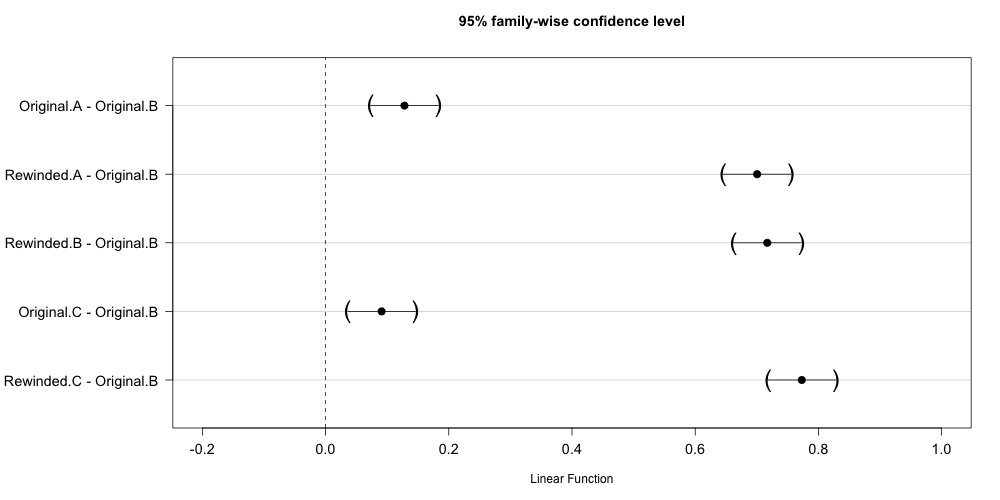
\includegraphics[width=\textwidth]{../figs/motors_mcpDun.png}};
\end{tikzpicture}
\end{ftstf}

%=====

\begin{ftst}
{Example: Electrical current in motors}
{Final Considerations}
For this example, the engineers would have now enough data to draw recommendations. For example, the data clearly shows that rewinded motors result in much larger currents drawn, which results in extra operational and structural (wiring, protection equipment, etc.) costs.
\vone
The engineers will factor economic and performance factors to reach conclusions about whether they should start gradually replacing all ventilation motors for new ones from manufacturer B, and whether it is better to fix or scrap the motors in need of rewinding.
\end{ftst}

%=====

\begin{ftst}
{General Factorial Designs}
{Experiments with more than 2 factors}
In the general case, the factorial design assumes:

\bitems \textit{a} levels of the factor \textbf{A};
\item \textit{b} levels of the factor \textbf{B};
\item \textit{c} levels of the factor \textbf{C};
\item\ldots
\eitem
\vhalf
If we consider an experiment with $n\geq 2$ replicates, the total number of observations required is given by $abc\ldots n$;
\lfr{It is actually possible to design an experiment with a single replicate (particularly for larger designs).  This will be discussed later.}
\end{ftst}

%=====

\begin{ftst}
{General Factorial Designs}
{Experiments with more than 2 factors}
The modeling and analysis of these experiments are easily obtained from the generalization of the design with 2 factors. For example, for 3 factors we have:
\begin{columns}
\column[T]{0.15\textwidth}
\column[T]{0.2\textwidth}
\begin{align*} y_{ijkl} &= \mu\\
&+ \tau_i + \beta_j + \gamma_k\\
&+(\tau\beta)_{ij} + (\tau\gamma)_{ik} + (\beta\gamma)_{jk}\\
&+ (\tau\beta\gamma)_{ijk}\\
&+ \epsilon_{ijkl}\\
&i=1,\ldots,a;\\
&j=1,\ldots,b;\\
&k=1,\ldots,c;\\
&l=1,\ldots,n;
\end{align*}
\column[T]{0.5\textwidth}
\begin{align*} &\longleftarrow\mbox{Grand mean}\\
&\longleftarrow\mbox{Main effects}\\
&\longleftarrow\mbox{2nd order interactions}\\
&\longleftarrow\mbox{3rd order interaction}\\
&\longleftarrow\mbox{Residual}\\
\end{align*}
\column[T]{0.15\textwidth}
\end{columns}
\end{ftst}

%=====

\begin{ftst}
{General Factorial Designs}
{Sum of squares: total and main effects}
\begin{align*}
SS_T &= \sum\limits_{i=1}^{a}\sum\limits_{j=1}^{b}\sum\limits_{k=1}^{c}\sum\limits_{l=1}^{n}{y_{ijkl}^2} - \frac{y_{\cdot\cdot\cdot\cdot}^2}{abcn}\\
SS_A &=\frac{1}{bcn}\sum\limits_{i=1}^{a} {y_{i\cdot\cdot\cdot}^2} - \frac{y_{\cdot\cdot\cdot\cdot}^2}{abcn}\\
SS_B &=\frac{1}{acn}\sum\limits_{j=1}^{b} {y_{\cdot j\cdot\cdot}^2} - \frac{y_{\cdot\cdot\cdot\cdot}^2}{abcn}\\
SS_C &=\frac{1}{abn}\sum\limits_{k=1}^{c} {y_{\cdot\cdot k\cdot}^2} - \frac{y_{\cdot\cdot\cdot\cdot}^2}{abcn}\\
\end{align*}
\end{ftst}

%=====

\begin{ftst}
{General Factorial Designs}
{Sum of squares: 2nd order interactions}
\begin{align*}
SS_{AB} &=\frac{1}{cn}\sum\limits_{i=1}^{a}\sum\limits_{j=1}^{b}{y_{ij\cdot\cdot}^2} - \frac{y_{\cdot\cdot\cdot\cdot}^2}{abcn} -SS_A-SS_B\\
SS_{AC} &=\frac{1}{bn}\sum\limits_{i=1}^{a}\sum\limits_{k=1}^{c}{y_{i\cdot k\cdot}^2} - \frac{y_{\cdot\cdot\cdot\cdot}^2}{abcn} -SS_A-SS_C\\
SS_{BC} &=\frac{1}{an}\sum\limits_{j=1}^{b}\sum\limits_{k=1}^{c}{y_{\cdot jk\cdot}^2} - \frac{y_{\cdot\cdot\cdot\cdot}^2}{abcn} -SS_B-SS_C\\
\end{align*}
\end{ftst}

%=====

\begin{ftst}
{General Factorial Designs}
{Sum of squares: 3rd order interaction and residual}
\begin{align*}
SS_{ABC} = &\frac{1}{n}\sum\limits_{i=1}^{a}\sum\limits_{j=1}^{b}\sum\limits_{k=1}^{c}{y_{ijk\cdot}^2} - \frac{y_{\cdot\cdot\cdot\cdot}^2}{abcn}\\
&-SS_A -SS_B -SS_C\\&- SS_{AB} -SS_{AC} -SS_{BC}\\
& \\
SS_{E} = &SS_T \\&-SS_A -SS_B -SS_C\\&- SS_{AB} -SS_{AC} -SS_{BC}\\&-SS_{ABC}
\end{align*}
\end{ftst}

%=====

\begin{ftst}
{General Factorial Designs}
{Example: intraocular lenses}
The standard surgical intervention for the treatment of cataracts consists in the removal of the crystalline lens and implantation of an artificial intraocular lens (IOL). IOLs are generally manufactured using a high precision CNC lathe, in which a circular piece of biocompatible material is carved to the desired lens shape with a diamond cutting tool.
\begin{tikzpicture}[remember picture,overlay]
\node[anchor=south east,yshift=36pt,xshift=5pt] at (current page.south east) {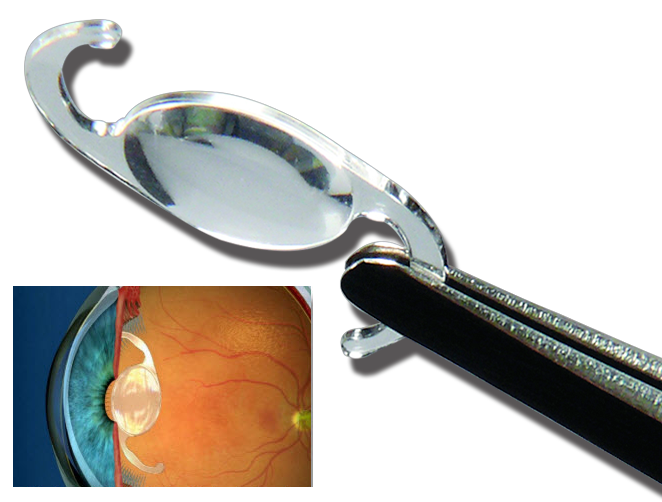
\includegraphics[width=0.45\textwidth]{../figs/lens02.png}};
\end{tikzpicture}

\lfr{Adapted from L.M. Carvalho e D.F. Filgueiras' course project for the Design and Analysis of Experiments Course, PPGEE-UFMG, June 2013. The data used in this example is not necessarily the original one.}
\lfr{Eye image: \url{http://www.peruenvideos.com/implante-lentes-intraoculares-curacion-cataratas/}}
\lfr{Lens image: \url{http://www.allaboutvision.com/conditions/iols.htm}}
\end{ftst}

%=====

\begin{ftst}
{General Factorial Designs}
{Example: intraocular lenses}
Before being marketed each lens is tested for the compliance of their optical properties, and the ones that fail to meet the required specifications are discarded.
\vone
Based on their knowledge of this process, two engineers designed an experiment for the preliminary investigation of the influential factors on the percentage of lenses that meet the specifications.
\vone
Three factors were selected for this preliminary study, each one with two levels. The resources allocated to the study were enough for the execution of exactly eight batches of lenses - in other words, a \textit{single replicate} for each combination of levels.
\end{ftst}

%=====

\begin{ftst}
{General Factorial Designs}
{Example: intraocular lenses}
Factors and levels:
\bitems Lathe time (in minutes): [$2.35; 3.15$];
\item Polishing time (in days): [$5; 7$];
\item Age of the cutting tool (in cycles): [$\approx 400; \approx 1200$];
\eitem
\vhalf
For each combination of levels a batch of 30 lenses was produced, and the proportion of lenses in conformity with specification was recorded  as the response variable.
\vhalf
The experiment was conducted in a completely randomized way, with partial blinding (lathe operators and technical inspectors did not know which level combination they were dealing with). 
\vhalf
The significance level was set as $\alpha=0.05$, and the researchers were interested in detecting any effects equal or larger than $0.1$ with a power of $0.8$.
\end{ftst}

%=====

\begin{ftstf}
{General Factorial Designs}
{Example: intraocular lenses}
Since there is only one replicate, there are not enough degrees of freedom to calculate $MS_E$. Consequently, the test of hypotheses becomes unfeasible.

\begin{rcode}
> data <- read.table("../data files/lio.txt", header = TRUE)

> model<-aov(Conf.rate ~ .^3, data = data)
> summary(model)
                                        Df Sum Sq Mean Sq
CNCTime.min                              1 0.5151  0.5151
PolTime.days                             1 0.0861  0.0861
ToolAge.cycles                           1 0.0105  0.0105
CNCTime.min:PolTime.days                 1 0.0036  0.0036
CNCTime.min:ToolAge.cycles               1 0.0001  0.0001
PolTime.days:ToolAge.cycles              1 0.0001  0.0001
CNCTime.min:PolTime.days:ToolAge.cycles  1 0.0036  0.0036
\end{rcode}
\end{ftstf}

%=====

\begin{ftst}
{General Factorial Designs}
{Model simplification}
To perform the test we need some degrees of freedom for the error term. In cases with single replicates, the most usual way of doing this is by discarding low-influence terms from the model. But which ones should be discarded?
\vone
A good way to proceed in these cases is to start by removing the highest-order interactions from the model, so that these terms are absorbed for the calculation of $MS_E$. 
\vone
This heuristic is based on the \textit{sparsity principle}, which states that most systems are dominated by main effects and low-order interactions;
\end{ftst}

%=====

\begin{ftst}
{General Factorial Designs}
{Model simplification}
A qualitative way of verifying the possibility of excluding some effects is the examination of a plot known as \textit{Daniel's effects plot}, which consists on plotting effect estimators obtained from a \textit{saturated} model on a normal QQ plot.
\vone
Strong effects will appear as outliers, while weak or insignificant effects will apper around the expected Normal line. By examining this plot we can obtain a simplified model, containing only the relevant effects.
\vone
Daniel plots work only in designs with only 2 levels per factor ($2^k$ \textit{designs}).
\lfr{For a more general effects plot, check Whitcomb and Oehlert (2007), \textit{Graphical Selection of Effects in General Factorials}: \url{http://goo.gl/6dw7dn}}
\end{ftst}

%=====

\begin{ftstf}
{Example: intraocular lenses}
{Model simplification}
\begin{rcode}
> effect.est <- as.numeric(model$effects[-1])
> qq.text    <- rownames(summary.aov(model)[[1]])
> qq.obj     <- qqnorm(effect.est, datax = TRUE, ...)
> qqline(effect.est, datax = TRUE)
> text(qq.obj$x, qq.obj$y, labels = qq.text,...)
\end{rcode}
\vhalf
The effects plot suggests that the higher\\
order effects have little influence over\\
the response variable;
\vhalf
Factor \textbf{CNCTime} seems to be\\
the most important, with \textbf{PolTime}\\
also a possibly interesting effect.
\begin{tikzpicture}[remember picture,overlay]
\node[anchor=south east,yshift=0pt,xshift=5pt] at (current page.south east) {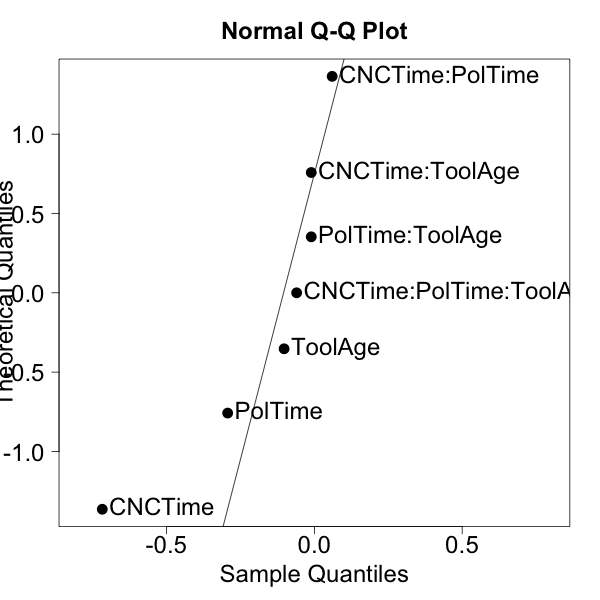
\includegraphics[width=0.48\textwidth]{../figs/lio_Daniel.png}};
\end{tikzpicture}
\end{ftstf}

%=====

\begin{ftstf}
{Example: intraocular lenses}
{Model simplification}
Discarding the interaction effects, we can suggest a simplified model:
\begin{rcode}
> model2 <- aov(Conf.rate ~ ., data = data)
> summary(model2)
            Df Sum Sq Mean Sq F value   Pr(>F)    
CNCTime      1 0.5151  0.5151 276.570 7.66e-05 ***
PolTime      1 0.0861  0.0861  46.235  0.00244 ** 
ToolAge      1 0.0105  0.0105   5.644  0.07634 .  
Residuals    4 0.0074  0.0019                     

> summary.lm(model2)$r.squared
[1] 0.9879681

> shapiro.test(model2$residuals)
W = 0.9271, p-value = 0.4902
\end{rcode}
\end{ftstf}

%=====

\begin{ftstf}
{Example: intraocular lenses}
{Exploring Specific Differences}
\begin{rcode}
> summary(glht(model2, linfct = mcp(CNCTime = "Tukey")))
Linear Hypotheses:
                  Estimate Std. Error t value Pr(>|t|)    
short - long == 0 -0.50750    0.03052  -16.63 7.66e-05 ***

> summary(glht(model2, linfct = mcp(PolTime = "Tukey")))
Linear Hypotheses:
                  Estimate Std. Error t value Pr(>|t|)   
short - long == 0 -0.20750    0.03052    -6.8  0.00244 **
\end{rcode}
\end{ftstf}

%=====

\begin{ftstf}
{Example: intraocular lenses}
{Exploring Specific Differences}
\begin{rcode}
> library(effects)
> lio.effs <- allEffects(model2)
> plot(lio.effs)
\end{rcode}
\begin{tikzpicture}[remember picture,overlay]
\node[anchor=south east,yshift=0pt,xshift=5pt] at (current page.south east) {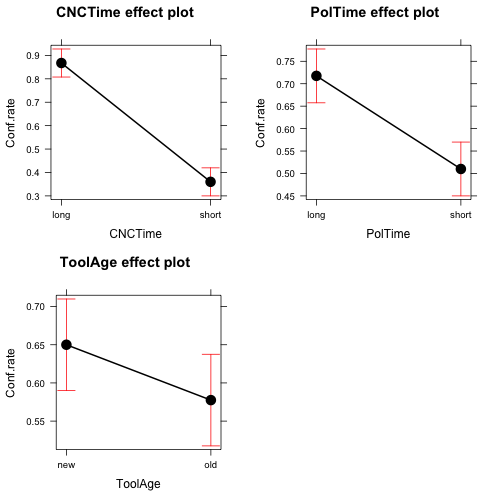
\includegraphics[width=0.6\textwidth]{../figs/lio_effs.png}};
\end{tikzpicture}
\end{ftstf}

%=====

\begin{ftst}
{Example: intraocular lenses}
{Some conclusions}
The effect of greatest impact on the quality of the process if the lathe time. The proportion of lenses in conformity with the specifications goes from $0.36$ to $0.87$, which strongly suggests the use of larger lathe times as a good strategy.
\vone
The polishing time  also presented a significant impact, with a jump from $0.51$ (5 days) to $0.71$ (7 days) on the proportion of compliant lenses.
\vone
No significant difference was detected between ``old'' and ``new'' cutting tools. This may have been due to an absence of effect, or due to the low sample size employed in this test. 
\vone
It is probably interesting to explore CNC lathe times further, and to include manufacturing cost considerations into this discussion.
\end{ftst}

%=====

\begin{ftst}
{General Factorial Designs}
{Some considerations about blocking}
The inclusion of blocking variables in factorial designs essentially as simple as the single-factor case.
\vone
The RCBD will contain one full experimental replicate per block. The modeling and analysis aspects can be easily derived from the last two chapters.
\vone

\end{ftst}

\begin{ftst}
{Bibliography}
{\ }
\scriptsize
\textbf{Required reading}

\benums D.C. Montgomery, G.C. Runger, \textit{Applied Statistics and Probability for Engineers}, 3rd ed., 2003 - Chapter 14;
\item P. Hoff, \textit{Applied Statistics and Experimental Design}, Chapter 6 (Factorial Designs), \url{http://goo.gl/NiyVCX} 
\eenum

\textbf{Recommended reading}
\benums R. Feynman, \textit{Surely you're joking, Mr. Feynman}, W.W. Norton\&Company, 1997.
\item H. Wickham, \textit{ggplot2: Elegant Graphics for Data Analysis}, Springer 2009.
\eenum
\end{ftst}

%=====

\begin{ftstf}{About this material}{Conditions of use and referencing}
\centering\footnotesize This work is licensed under the Creative Commons CC BY-NC-SA 4.0 license\\(Attribution Non-Commercial Share Alike International License version 4.0).\\
\vhalf
\url{http://creativecommons.org/licenses/by-nc-sa/4.0/}\\
\vone
\footnotesize Please reference this work as:\\
\footnotesize \flushleft Felipe Campelo (2015), \textit{Lecture Notes on Design and Analysis of Experiments}.\\Online: {\scriptsize\url{https://github.com/fcampelo/Design-and-Analysis-of-Experiments}}\\
Version 2.11, Chapter 12; Creative Commons BY-NC-SA 4.0.\\

\begin{Verbatim}[fontsize=\tiny]
    @Misc{Campelo2015-01,
      title={Lecture Notes on Design and Analysis of Experiments},
      author={Felipe Campelo},
      howPublished={\url{https://github.com/fcampelo/Design-and-Analysis-of-Experiments}},
      year={2015},
      note={Version 2.11, Chapter 12; Creative Commons BY-NC-SA 4.0.},
    }
\end{Verbatim}

\begin{tikzpicture} [remember picture,overlay]
\node[anchor=south,yshift=0pt] at (current page.south){ \includegraphics[width=.2\textwidth]{../figs/CCSomerights.png}};
\end{tikzpicture}
\end{ftstf}


\end{document}